\chapter[Resultados e Análise dos Resultados]{Resultados e Análise dos Resultados}

\section{Consumo de Combustível}
A tabela \ref{tabela_resultados} apresenta os resultados do experimento com o motor operando somente com gasolina, a duplo combustível com o gaseificador a topo aberto e a topo fechado. 

\begin{table}[h]
	\centering
	\caption{Resultados do experimento. (Fonte: autoria própria)}
	\begin{tabular}{|c|c|c|c|c|c|}
		\hline
		Combustível & Rotação & Tempo & Posição & Pressão & Consumo	\\
		& do Motor & de Injeção & da Borboleta & Coletor & \\
		& (rpm) & (ms) & (graus) & (mmHg) & (L/h)\\
		\hline
		\multirow{12}{4.5cm}{Gasolina}
		& 926 & 0,52 & 14 & 388 & 1,63 x 10\textsuperscript{-1}\\
		& 969 & 0,55 & 14 & 355 & 1,80 x 10\textsuperscript{-1}\\
		& 984 & 0,53 & 14 & 352 & 1,76x 10\textsuperscript{-1}\\
		& 3597 & 0,54 & 24 & 283 & 6,57 x 10\textsuperscript{-1} \\
		& 4007 & 0,44 & 24 & 460 & 5,96 x 10\textsuperscript{-1}\\
		& 4038 & 0,68 & 24 & 470 & 9,28 x 10\textsuperscript{-1}\\
		& 4046 & 0,49 & 24 & 271 & 6,70 x 10\textsuperscript{-1}\\
		& 4056 & 0,66 & 24 & 259 & 9,05 x 10\textsuperscript{-1}\\
		& 4061 & 0,66 & 24 & 450 & 9,06 x 10\textsuperscript{-1}\\
		& 4071 & 0,65 & 24 & 259 & 8,94 x 10\textsuperscript{-1}\\
		& 4107 & 0,68 & 24 & 259 & 9,44 x 10\textsuperscript{-1}\\
		\hline
		\multirow{12}{4.5cm}{Gasolina + syngas (Topo aberto)}
		& 3532 & 0,49 & 24 & 283 & 5,85 x 10\textsuperscript{-1}\\
		& 3579 & 0,48 & 24 & 280 & 5,81 x 10\textsuperscript{-1}\\
		& 3656 & 0,49 & 24 & 280 & 6,06 x 10\textsuperscript{-1}\\
		& 3838 & 0,61 & 24 & 259 & 7,91 x 10\textsuperscript{-1}\\
		& 4009 & 0,68 & 24 & 259 & 9,08 x 10\textsuperscript{-1}\\
		& 4021 & 0,67 & 24 & 262 & 9,11 x 10\textsuperscript{-1}\\
		& 4035 & 0,65 & 24 & 259 & 8,86 x 10\textsuperscript{-1}\\
		& 4038 & 0,64 & 24 & 259 & 8,74 x 10\textsuperscript{-1}\\
		& 4047 & 0,64 & 24 & 259 & 8,75 x 10\textsuperscript{-1}\\
		& 4061 & 0,65 & 24 & 259 & 8,92 x 10\textsuperscript{-1}\\
		& 4162 & 0,68 & 24 & 265 & 9,57 x 10\textsuperscript{-1}\\
		\hline
		\multirow{12}{4.5cm}{Gasolina + syngas (Topo fechado)}
		& 887 & 0,65 & 14 & 409 & 1,95 x 10\textsuperscript{-1}\\
		& 893 & 0,65 & 14 & 466 & 3,68 x 10\textsuperscript{-1}\\
		& 926 & 0,88 & 14 & 388 & 2,75 x 10\textsuperscript{-1}\\
		& 927 & 0,71 & 14 & 415 & 2,22 x 10\textsuperscript{-1}\\
		& 2767 & 0,81 & 22 & 301 & 7,58 x 10\textsuperscript{-1}\\
		& 2794 & 0,50 & 22 & 301 & 4,72 x 10\textsuperscript{-1}\\
		& 2805 & 1,02 & 22 & 298 & 9,67 x 10\textsuperscript{-1}\\
		& 2858 & 0,52 & 22 & 289 & 5,02 x 10\textsuperscript{-1}\\
		& 2868 & 0,68 & 23 & 301 & 6,59 x 10\textsuperscript{-1}\\
		& 2875 & 0,63 & 22 & 289 & 6,12 x 10\textsuperscript{-1}\\
		& 3026 & 0,81 & 23 & 292 & 8,28 x 10\textsuperscript{-1}\\	
		\hline
	\end{tabular}
	\label{tabela_resultados}
\end{table}	

A figura \ref{grafico_consumo} mostra um gráfico representando o consumo do motor com as diferentes configurações de combustível analisadas.

\begin{figure}[!htb]
	\centering
	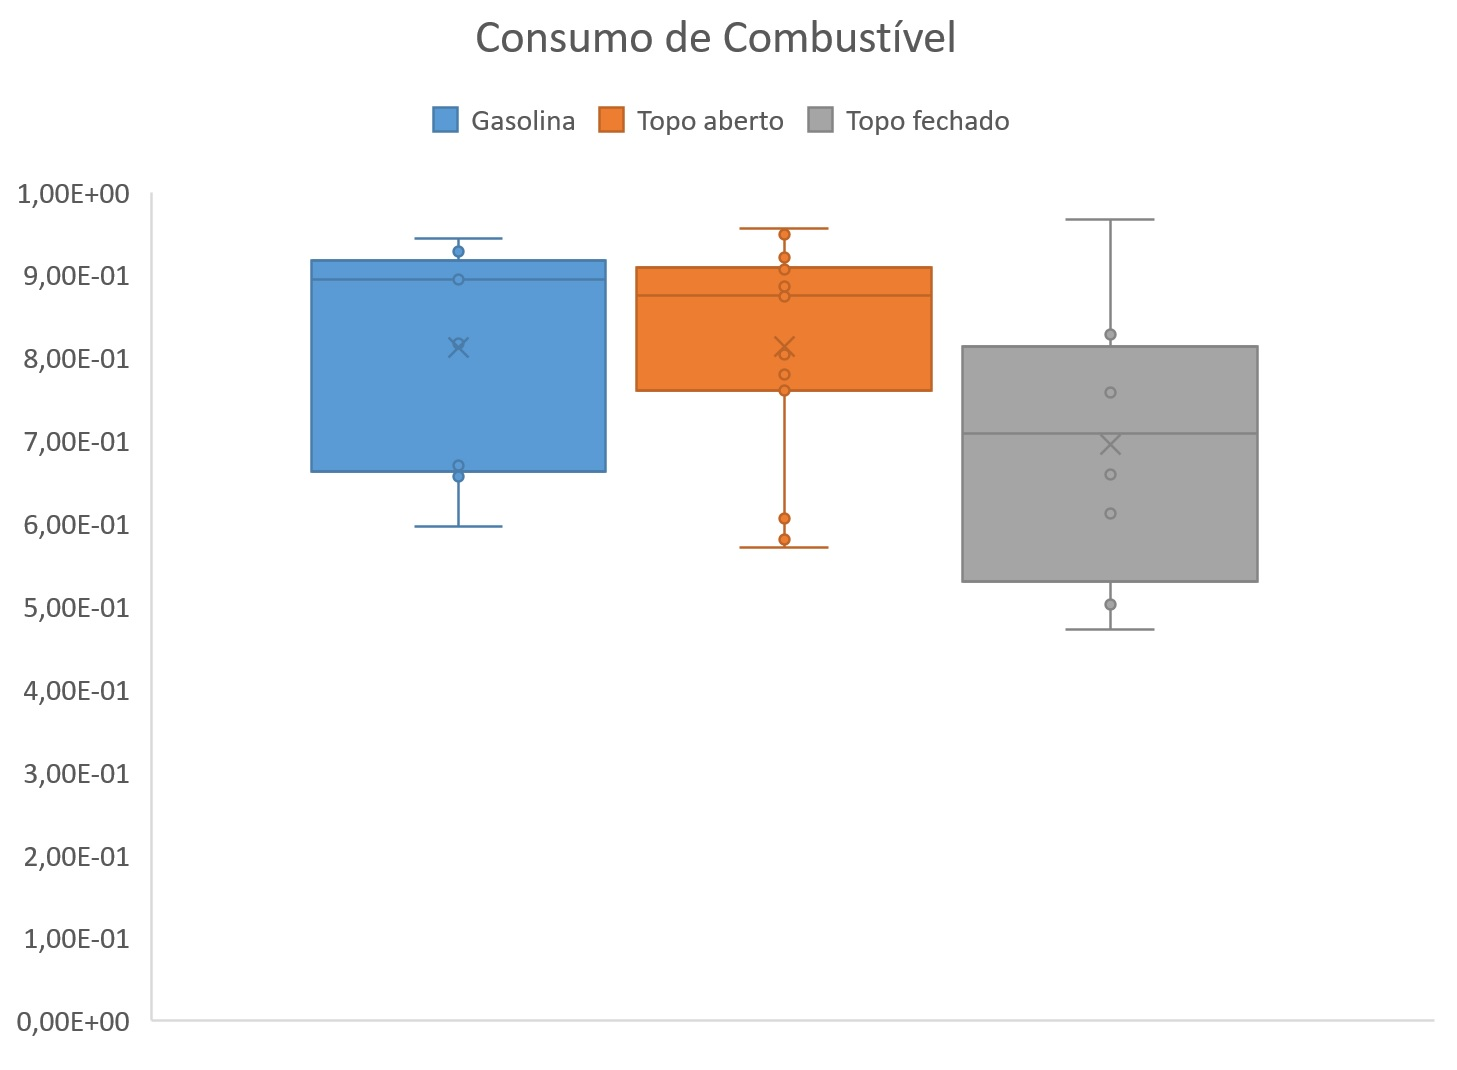
\includegraphics{Figuras/consumo_combustivel}
	\caption{Consumo de Combustível}
	\label{grafico_consumo}
\end{figure}

Trabalhando a duplo combustível com topo aberto, o abatimento no consumo de gasolina  com a adição do gás de síntese é mínima. Ao pressurizar o sistema trabalhando com o topo fechado, essa diferença de consumo se mostra mais evidente, chegando a uma redução de 14,4\%.

Esse resultado insatisfatório do gás de síntese no consumo do motor pode ser explicado pela perda de carga na mangueira de entrada de gases, uma vez que esta apresentava diâmetro muito pequeno e, de acordo com a fórmula de Darcy-Weibasch, a perda de carga e o diâmetro da tubulação são inversamente proporcionais, ou seja, quanto menor o diâmetro, maior a perda de carga.

\begin{equation} \label{darcy-weibasch}
 h\textsubscript{f} = f\textsubscript{d}\frac{L}{D}\frac{\rho V^2}{2}
\end{equation}

Onde f\textsubscript{D} é o coeficiente de atrito, L é o comprimento, D é o diâmetro, $\rho$ é massa específica e V é a velocidade.

\section{Geração de Energia}

A tabela \ref{tabela_resultados_2} mostra o resultado dos cálculos realizados com os dados coletados durante o experimento. Considerou-se os cálculos com 200 gramas de biomassa a topo fechado consumida durante o tempo \textit{t} ocupando metade da altura do reator.

\begin{table}[h]
	\centering
	\caption{Cálculos realizados com os dados coletados. (Fonte: autoria própria)}
	\begin{tabular}{|l|c|c|c|}
		\hline
		Variável & Símbolo & Valor & Equação \\
		\hline
		
		Área da seção transversal & A\textsubscript{g} & 0,01227m\textsuperscript{2} & - \\
		
		Altura da coluna de biomassa & h$_b$ & 0,25m & -\\
		
		Massa específica aparente & $\rho$\textsubscript{ap} & 65,2 kg/m\textsuperscript{3} & - \\
		
		Tempo de comsumo da biomassa & t & 9min ou 0,15h & -\\
		
		Vazão mássica de biomassa & $\dot{m}$\textsubscript{biomassa} & 1,33 kg/h & Eq. \ref{vazao_biomassa_PCI}\\
		
		Taxa específica de processamento do reator & $\psi$ & 105 kg/m\textsuperscript{2}h & Eq. \ref{taxa_reator}\\
		
		\rowcolor{lightgray} Poder Calorífico do syngas & PCI\textsubscript{gas} & 5,07 MJ/Nm\textsuperscript{3} & Eq. \ref{PCI_Tiangco}\\
		
		Vazão volumétrica do bagaço & $\dot{Q}$\textsubscript{bagaço} & 0,024m\textsuperscript{3}/h & Eq. \ref{qdot_bagaco}\\
		
		Vazão volumétrica do ar & $\dot{Q}$\textsubscript{ar} & 1,2Nm\textsuperscript{3}/h & -\\
		
		Vazão volumétrica do gás de síntese & $\dot{Q}$\textsubscript{syngas} & 1,224Nm\textsuperscript{3}/h & Eq. \ref{balanco_massa}\\
		
		\rowcolor{lightgray} Potência térmica & P\textsubscript{t} & 1.724 W & Eq. \ref{potencia_termica}\\
		
		\hline
\end{tabular}
\label{tabela_resultados_2}
\end{table}	

Com base nas equações \ref{potencia_eixo} e \ref{potencia_eletrica}, traça-se um gráfico com as potências de eixo e potência elétrica que podem ser geradas em função da potência térmica do syngas, assumindo eficiências entre 10\% e 90\% para $\eta$\textsubscript{motor} e 90\% para $\eta$\textsubscript{g}.

\begin{figure}[!htb]
	\centering
	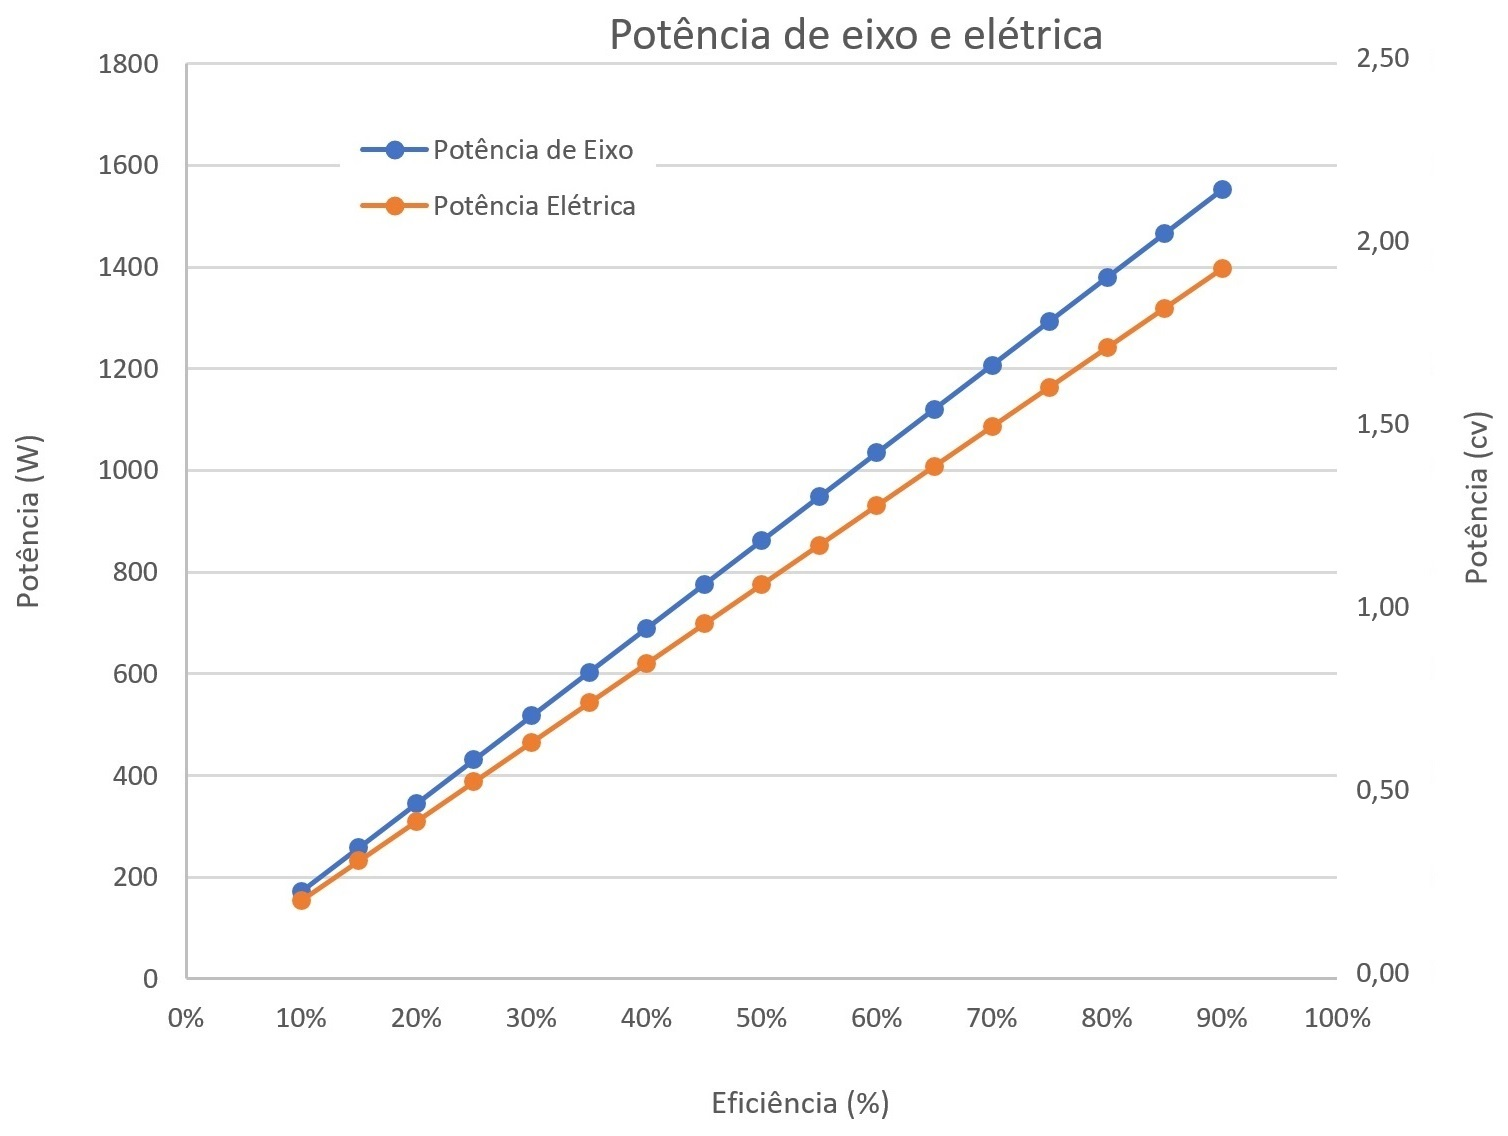
\includegraphics[width=13.5cm]{Figuras/grafico_potencia_eficiencia}
	\caption{Gráfico das potências de eixo e elétrica.}
	\label{grafico_potencia_eficiencia}
\end{figure}

Segundo \cite{brunetti2012}, a máxima eficiência térmica de um motor de combustão interna é a eficiência do ciclo de Carnot para as condições máximas e mínimas de temperatura neste tipo de motor, resultando numa eficiência máxima de 57,2\%. Um MCI deve ter eficiência térmica abaixo deste valor.

Portanto, um motor a combustão genérico com eficiência de até 57\%, trabalhando com gás de síntese do bagaço de cana com uma potência térmica de 1.724W, sem condiserar as demais perdas do sistema, seria capaz de movimentar uma moenda de cana de até 1,3cv acoplada ao seu eixo. Acoplando um gerador, o conjunto moto-gerador supriria um motor elétrico de até 1,2cv.

Na tabela \ref{tabela_moendas}, seguem as especificações de diferentes modelos de moenda da marca Maqtron, de acordo com seu catálogo.

\begin{table}[h]
	\centering
	\caption{Tabela de moendas de cana marca Maqtron \cite{catalogo2016}}
	\begin{tabular}{|c|c|c|}
	\hline
	\rowcolor{lightgray}\textbf{Modelo Moenda} & \textbf{Motor elétrico indicado} & \textbf{Motor estacionário indicado} \\
	\rowcolor{lightgray} & \textbf{[CV]} & \textbf{[CV]} \\
	\hline
	Cana Express Hobby & 1/2 & - \\
	Cana Shop 60 & 1/2 & - \\
	Cana Shop 140 & 1 & - \\
	Cana Shop 200 & 2 & - \\
	Cana Shop Estacionária & - & 3,5 - 5,0 \\
	B-721 Turbo & 1,5 - 2,0 & 3,5 \\
	B-722 Turbo & 1,2 - 2,0 & 3,5 \\
	M-700 & 1 & - \\
	B-728 & 1/2 & - \\
	B-730 & 5 a 7,5 & 8 a 12 \\
	B-723 & 1/2 - 1,0 & - \\
	\hline
	\end{tabular}
	\label{tabela_moendas}
\end{table}	

De acordo com a tabela \ref{tabela_moendas}, para esses modelos de moenda, seria necessário um motor a combustão com potência de eixo mínima de 3,5cv. Portanto, um motor a combustão necessitaria trabalhar a duplo combustível para suprir a demanda de potência de tais moendas, uma vez que a energia do gás de síntese sozinho não é capaz de fornecer potência suficiente, de acordo com os cálculos teóricos.

O motor a combustão da Fiat que foi acoplado ao reator neste experimento é capaz de fornecer \textcolor{red}{XW} de potência de eixo trabalhando a duplo combustível com o gaseificador a topo fechado, de acordo com a equação \textcolor{red}{equação}. Portanto, ele tem condições de fornecer a potência de eixo demandada pela moenda trabalhando a duplo combustível, porém, devem ser feitos ajustes na configuração do aparato experimental para que seja diminuída a perda de carga do sistema e possa haver participação significativa do gás de síntese na conversão da energia, uma vez que o objetivo é o incentivo ao uso da biomassa como fonte energética.

Um moto-gerador com uma eficiência de 70\%, ou superior, seria capaz de suprir a potência de um motor elétrico de 1,5cv trabalhando somente com gás de sítnese, sem considerar perdas. Para as moendas que demandam valores de 2cv e acima, tal moto-gerador necessitaria trabalhar a duplo combustível. Para moendas pequenas que demandam potência do motor elétrico de 1/2 cv, seria necessário um moto-gerador com eficiência mínima de 23,5\%.

		